\subsection{Remanufacturing and Refurbishing: \textit{Description}}

\subsubsection{Definition}
Remanufacturing involves disassembling the full structure of a multi-component product, inspecting, cleaning, repairing, or replacing necessary parts, and reassembling it to its original state or better. This process can include both reused and new components, aiming to achieve a quality level that meets or exceeds the new product~\cite{reike2018rex, sihvonena2015reman, zhang2012reman}.

Refurbishing, often confused with remanufacturing, is the process where the overall structure of a large multi-component product remains intact, while components are replaced or repaired, resulting in an overall ‘upgrade’ of the product. It aims to bring the product up to a specified quality, possibly incorporating newer, more advanced components~\cite{reike2018rex}.

\boxparameter{Remanufacturing and Refurbishing}{Stable}{Stable}{Strong increase}

\subsubsection{Context}
Remanufacturing and refurbishing are essential strategies in the circular economy, aimed at extending product lifecycles and reducing waste. They are particularly relevant in the medium loops (R4-R6) of product recovery, where they serve as business activities indirectly linked to the consumer~\cite{eu2015reman}.

\subsubsection{International and European Trends}
Remanufacturing is gaining momentum globally, particularly in the U.S. and Europe. Governments are legislating manufacturers to assume responsibility for their products post-use, emphasizing recyclability and waste reduction. The market for environmentally friendly products, valued at over USD 200 billion, is driving corporations to adopt remanufacturing and other green practices~\cite{mitra2005reman,irp2018manufacturing}.

\subsubsection{Implementation in EU Law}
EU laws increasingly mandate manufacturers to engage in product recovery, including remanufacturing. This aligns with the EU's broader goals of sustainable development, resource efficiency, and transitioning to a circular economy~\cite{eu2015reman,eu2019greendeal}.

\subsubsection{Economic Scale and Regional Focus in Europe}
The remanufacturing industry in Europe generates around €30bn in turnover and employs about 190,000 people. Key regions like Germany, the UK, Ireland, France, and Italy have significant remanufacturing activities. Germany leads in remanufacturing turnover, particularly in aerospace, automotive, and heavy-duty off-road (HDOR) sectors~\cite{eu2015reman}.

\subsubsection{Benefits and Risks}
\begin{description}
    \item[Environmental Benefits and Risks:] Remanufacturing significantly reduces environmental impact by conserving raw materials and energy, while risks may include the potential for resource-intensive processes if not efficiently managed.
    \item[Manufacturers' Perspective:] For manufacturers, remanufacturing offers economic benefits, with costs typically 40–60\% lower than manufacturing new products. It also enhances corporate image and competitive advantage in a market increasingly sensitive to environmental concerns~\cite{mitra2005reman}.
    \item[Broader Economic and Environmental Implications:] Remanufacturing contributes to a sustainable economy, offering a less resource-intensive alternative to new production. It supports employment, innovation, and reduces dependency on raw material extraction.
\end{description}

\subsubsection{Benefits and Risks}
\begin{description}
    \item[Environmental Benefits and Risks:] Remanufacturing significantly reduces environmental impact by conserving raw materials and energy. However, risks may include the potential for resource-intensive processes, especially if not managed efficiently, and the need for effective sorting and inspection policies to decide on the remanufacturability of returned products~\cite{singhal2020reman}.

    \item[Manufacturers' Perspective:] For manufacturers, remanufacturing offers economic benefits, with costs typically 40–60\% lower than manufacturing new products. It also enhances corporate image and competitive advantage in a market increasingly sensitive to environmental concerns. Additionally, manufacturers' identity, brand reputation, and technological capabilities play a crucial role in the success of remanufacturing initiatives~\cite{mitra2005reman, singhal2020reman}.

    \item[Broader Economic and Environmental Implications:] Remanufacturing contributes to a sustainable economy, offering a less resource-intensive alternative to new production. It supports employment, innovation, and reduces dependency on raw material extraction. Key factors such as government regulations, collection strategies, and public awareness about environmental benefits are crucial in promoting remanufacturing. Moreover, design for remanufacturing and skilled labor are essential for efficient remanufacturing processes~\cite{singhal2020reman}.

    \item[Market Dynamics:] Factors like consumer purchase intentions, pricing strategies, and the fear of cannibalization significantly influence the market for remanufactured products. Consumers' willingness to return used products and their perception of remanufactured products also play a crucial role in shaping the remanufacturing market~\cite{singhal2020reman}.

    \item[Regulatory and Strategic Aspects:] Government regulations, such as take-back laws and extended producer responsibility, incentivize remanufacturing. Strategic elements like inventory control, scheduling, and material matching are vital for operational efficiency in remanufacturing. Management prescience is required to spearhead remanufacturing business and maintain circularity in the economy~\cite{singhal2020reman}.
\end{description}

 \autoref{fig:remanufacturing} illustrates an example of a remanufacturing process (in this case, for vehicle components), highlighting the key steps and the inputs and outputs~\cite{zhao2021reman}.

\begin{figure}[ht!]
    \centering
    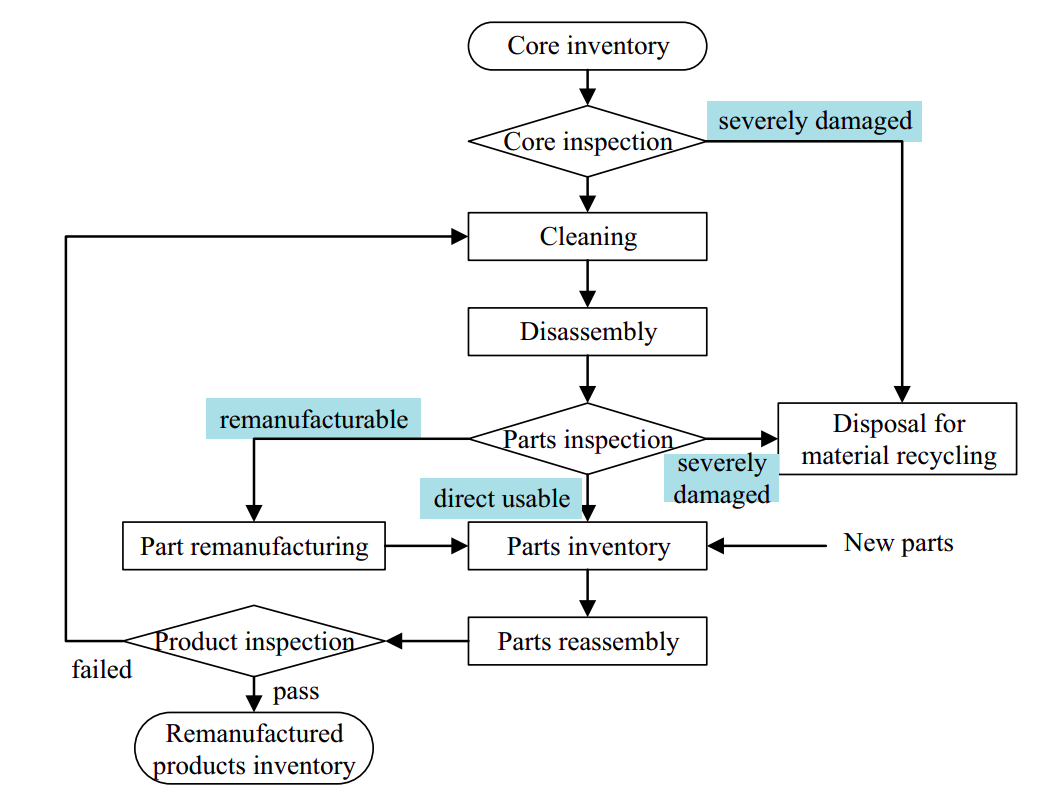
\includegraphics[width=\linewidth]{130quantification/internal/cei/zhao2021reman.png}
    \caption[An example of a generic remanufacturing process for vehicle components]{An example of a generic remanufacturing process for vehicle components~\cite{zhao2021reman}}
    \label{fig:remanufacturing}
\end{figure}
\FloatBarrier
\sectionEndlines
\clearpage


\subsubsection{Relevance of Remanufacturing and Refurbishing in FutuRaM's Waste Streams}

\wasteSubsubsecBATT
\begin{itemize}
    \item Electric Vehicle Batteries: Remanufacturing can involve replacing degraded cells or modules to extend their lifespan, thereby conserving lithium and cobalt.
    \item Laptop Batteries: Through remanufacturing, individual cells within the battery pack can be replaced or upgraded, enhancing the overall battery life and efficiency.
\end{itemize}

\wasteSubsubsecELV
\begin{itemize}
    \item Automotive Engines: Remanufacturing can include refurbishing engine components, such as pistons and bearings, to restore performance and efficiency.
    \item Transmission Systems: Rebuilding transmission systems with replaced or refurbished gears and bearings can significantly extend the life of the vehicle.
\end{itemize}

\wasteSubsubsecWEEE
\begin{itemize}
    \item Smartphones: Remanufacturing can involve replacing batteries, screens, and other components to restore them to like-new condition.
    \item Printers and Copiers: Components such as toner cartridges, drums, and fusers can be remanufactured to extend their service life and improve functionality.
\end{itemize}

\wasteSubsubsecCDW
\begin{itemize}
    \item Structural Steel Elements: In construction and demolition, steel beams and columns can be refurbished and reused in new construction projects.
    \item Wooden Beams and Flooring: Wooden elements can be remanufactured through processes like sanding, treating, and reinforcing for reuse in construction.
\end{itemize}


\sectionEndlines
\clearpage
